\subsubsection*{Integrali della forma}

\begin{itemize}
    \item $\displaystyle \int_{0}^{2\pi} R(\cos\theta,\, \sin\theta)d\theta$.\\
        Ponendo $z\equiv e^{i\theta} = \cos\theta+i\sin\theta$, si ha:
        \begin{enumerate}[label=(\roman*)]
            \item $\cos\theta = \frac{1}{2} (e^{i\theta}+e^{-i\theta}) = \frac{1}{2}(z+\frac{1}{z})$;
            \item $\sin\theta = \frac{1}{2i} (e^{i\theta}-e^{-i\theta}) = \frac{1}{2i}(z-\frac{1}{z})$;
            \item $d\theta = \frac{1}{iz}dz$.
        \end{enumerate}
        quindi
        \begin{align*}
            I&\equiv\int_{0}^{2\pi} R(\cos\theta,\, \sin\theta)d\theta \\
            &= \oint_{|z|=1}R\left(\frac{1}{2}\left(z+\frac{1}{z}\right),\ \frac{1}{2i}\left(z-\frac{1}{z}\right)\right)\frac{dz}{iz}  \\
            &\equiv \oint_{|z|=1} \widetilde{R}(z)dz  \\
            & = 2\pi i\sum_{k=1}^{N_{\text{int}}}\text{Res}[\widetilde{R}(z),z_k],
        \end{align*}
        essendo $z_k:\,k=1,\dots,N_{\text{int}}$ i poli di $\widetilde{R}(z)$ all'interno del cerchio $\Delta_1=\{z:\ |z|<1\}$.
        \begin{center}
        \resizebox{\columnwidth/3}{!}{
            \begin{tikzpicture}
                \draw[red,thick] (0,0) circle (2.5);
                \node[red, rotate=45] at (-2,2) {$\Delta_1 \circlearrowleft$};
                \filldraw[black] (1.8,1) circle (1pt) node[anchor=west]{$z_1$};
                \filldraw[black] (-0.5,1.7) circle (1pt) node[anchor=west]{$z_2$};
                \filldraw[black] (-1.8,0.5) circle (1pt) node[anchor=west]{$z_3$};
                \filldraw[black] (-2.9,-0.5) circle (1pt) node[anchor=west]{$z_4$};
                \node at (-2.9,-0.5) {$\times$};
                \node at (-2.8,0.2) {$-1$};
                \node at (2.8,0.2) {$1$};
                \filldraw[black] (-1.5,-1.7) circle (1pt) node[anchor=west]{$z_5$};
                \filldraw[black] (1,-0.7) circle (1pt) node[anchor=west]{$z_k$};
                \draw[>=latex, ->, black] (0,-3.5) -- (0,3.5) node[left, pos=1]{$\pim z$};
                \draw[>=latex, ->, black] (-3.5,0) -- (3.5,0) node[above, pos=1]{$\pre z$};
            \end{tikzpicture}
            }
        \end{center}

    \item $\displaystyle \int_{-\infty}^{+\infty} e^{iax}f(x)dx$. \\
        Se $f(z)$ è analitica 
        \begin{enumerate}[label=(\roman*)]
            \item \label{sopra} nel semipiano complesso superiore Im$(z)\ge0$, oppure
            \item \label{sotto} nel semipiano complesso inferiore Im$(z)\le0$,
        \end{enumerate}
        tranne che in un numero finito di p.ti singolari isolati $z_k$, con $k=1, \dots, N$, e se 
        \[
            \lim_{R\to\infty}\left(\max_{z\in C_R'}|f(z)|\right) = 0
        \]
        con $C_R'$ semicirconferenza di raggio $R$ e centro in $z=0$ \ref{sopra} nel piano complesso sup. ($C_R'=\{z:|z|=R,\, \pim(z)\ge 0\}$), oppure \ref{sotto} nel piano complesso inf. ($C_R'=\{z:|z|=R,\, \pim (z)\le 0\}$), cioé se $\exists \mu(R)$ t.c. 
        \[
            |f(z)|\le\mu(R)\,\text{per }|z|=R,\,\text{con }\mu(R)\xrightarrow[]{R\to\infty}0,
        \]
        allora si ha che
        \begin{enumerate}
            \item[\ref{sopra}] $\displaystyle\lim_{R\to+\infty}\int_{C_R'}e^{iaz}f(Z)dz=0$, per $a>0$;
            \item[\ref{sotto}] $\displaystyle\lim_{R\to+\infty}\int_{C_R'}e^{iaz}f(Z)dz=0$, per $a<0$;
        \end{enumerate}
        \begin{center}
            \resizebox{\columnwidth/3}{!}{
                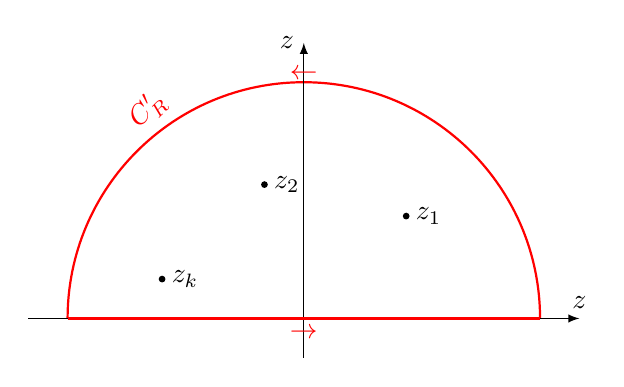
\begin{tikzpicture}
                    \draw[red, thick] (3, 0) arc (0:180:3) node[above, pos=0.7, rotate=45]{$C_R'$};
                    \filldraw[black] (1.3,1.3) circle (1pt) node[anchor=west]{$z_1$};
                    \filldraw[black] (-0.5,1.7) circle (1pt) node[anchor=west]{$z_2$};
                    \filldraw[black] (-1.8,0.5) circle (1pt) node[anchor=west]{$z_k$};
                    \draw[>=latex, ->, black] (0,-.5) -- (0,3.5) node[left, pos=1]{$\pim z$};
                    \draw[>=latex, ->, black] (-3.5,0) -- (3.5,0) node[above, pos=1]{$\pre z$};
                    \node[red, thick] at (0, 3.1) {$\leftarrow$};
                    \draw[red, thick] (-3,0) -- (3,0) node[below, pos=0.5]{$\rightarrow$};
                \end{tikzpicture}
            }
        \end{center}
    \item $\displaystyle \int_{0}^{\infty}x^\alpha f(x) dx$.\\ 
        Se valgono le ipotesi
        \begin{enumerate}[label=(\roman*)]
            \item il prolungamento analitico $f(z)$ della $f(x)$ è analitico ovunque tranne in un numero finito di p.ti singolari isolati $z_k$ ($k=1,\dots,N$);
            \item $z=0$ sia un p.to singolare eliminabile;
            \item vale la condizione 
            \[
                \max_{z\in C_R}|f(Z)|R^{\alpha+1}\xrightarrow[R\to\infty]{}0\, (\alpha\in\mathbb{R},\, 0<\alpha<1),
            \]
        \end{enumerate}
        allora
        \[
            \int_{0}^{\infty}x^\alpha f(x) dx = \frac{2\pi i}{1-e^{2\pi\alpha i}}\sum_{k=1}^{N}\text{Res}[z^\alpha f(z),\,z_k].
        \]
     
        
    %    Funzione python per calcolare i parametri degli archi per la figura a seguire
    %    import numpy as np
    %    def centri(start_deg, r1, r2):
    %        start_rad = start_deg * np.pi / 180
    %        x1 = r1 * np.cos(start_rad)
    %        y1 = r1 * np.sin(start_rad)
    %        centro1 = np.array([x1,y1])
    %        start_rad_piccolo = np.arcsin(y1/r2)
    %        x2 = r2 * np.cos(start_rad_piccolo)
    %        y2 = y1
    %        centro2 = np.array([x2,y2])
    %        start_deg_piccolo = start_rad_piccolo * 180 / np.pi
    %        stop_deg_piccolo = 360 - start_deg_piccolo
    %        stasto_piccolo = np.array([start_deg_piccolo, stop_deg_piccolo])
    %        return centro1, centro2, stasto_piccolo
      
        \begin{center}
            \resizebox{\columnwidth/3}{!}{
                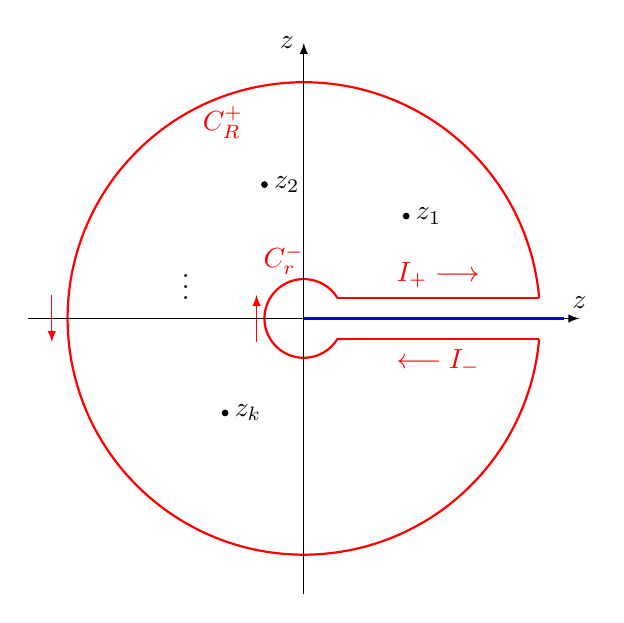
\begin{tikzpicture}
                    \draw[red, thick] (2.98858409, 0.26146723) arc (5:355:3) node[below, pos=0.3]{$C_R^+$};
                    \draw[red, thick] (0.42618645, 0.26146723) arc (31.5292956:328.47070432:0.5) node[above, pos=0.3]{$C_r^-$};
                    \draw[red, thick] (2.98858409,0.26146723) -- (0.42618645,0.26146723) node[above, pos=0.5]{$I_+\longrightarrow$};
                    \draw[red, thick] (2.98858409,-0.26146723) -- (0.42618645,-0.26146723) node[below, pos=0.5]{$\longleftarrow I_-$};
                    \filldraw[black] (1.3,1.3) circle (1pt) node[anchor=west]{$z_1$};
                    \filldraw[black] (-0.5,1.7) circle (1pt) node[anchor=west]{$z_2$};
                    \node at (-1.5, 0.5) {$\vdots$};
                    \filldraw[black] (-1,-1.2) circle (1pt) node[anchor=west]{$z_k$};
                    \draw[>=latex, ->, red] (-3.2,0.3) -- (-3.2,-.3);
                    \draw[>=latex, <-, red] (-.6,0.3) -- (-.6,-.3);
                    \draw[>=latex, ->, black] (0,-3.5) -- (0,3.5) node[left, pos=1]{$\pim z$};
                    \draw[>=latex, ->, black] (-3.5,0) -- (3.5,0) node[above, pos=1]{$\pre z$};
                    \draw[thick, blue] (0,0) -- (3.3,0);
                \end{tikzpicture}
            }
        \end{center}
        
    \item $\displaystyle \int_{0}^{+\infty}f(x) \log x dx$
        \begin{enumerate}
            \item[a')] Ipotizzando che il prolungamento analitico $f(z)$ di $f(x)$ sia una funzione analitica univoca ovunque tranne che in un numero finito di punti singolari isolati $z_k,\,k=1,\dots,N$, non giacenti su $\{z:\pim (z)=0\, e\, \pre (z)>0\} $ e che $z=0$ sia un p.to singolare eliminabile, si ha 
            \begin{gather*}
                \int_{0}^{+\infty}f(x)\  dx = \pre \left\{\frac{i}{2\pi}\sum_{k=1}^{N}\text{Res}[f(z)(\log z)^2,\, z_k]\right\};\\
                \int_{0}^{+\infty}f(x) \log x\ dx = \pim\left\{-\frac{i}{2}\sum_{k=1}^{N}\text{Res}[f(z)(\log z)^2,\, z_k]\right\}.
            \end{gather*}
            \item[b')] Nel caso in cui $f(x)$ sia pari ($f(-x)=f(x)$), si ha che
            \begin{align*}
                2\int_{0}^{+\infty}f(x) \log x dx + i\pi \int_{0}^{+\infty}f(x) dx =\\
                = 2\pi i \sum_{\pim z_k > 0}\text{Res}[f(z)\log z,\, z_k].
            \end{align*}
            Prendendone la parte reale e la parte immaginaria otteniamo gli integrali desiderati.
        \end{enumerate}

\end{itemize} 
